\documentclass{beamer}
%\usepackage{default}
\usetheme[progressbar=frametitle]{metropolis}


\usepackage[utf8]{inputenc} % per gli accenti
\usepackage{amsmath}
\usepackage{mathtools}
\usepackage{graphicx}
\usepackage{listings, inconsolata}
\usepackage{color}

\usepackage{media9}

\definecolor{mygray}{rgb}{0.9,0.9,0.9}
\lstset{backgroundcolor=\color{mygray}, 
	    tabsize=2, 
	    frame=lines,
		basicstyle=\ttfamily\footnotesize,
		keywordstyle=\bfseries,
		breaklines=true,
		keywordstyle=\color{blue}
}

\title {
	Turtlebot 3 Autonomous Driving
}
\author{Falezza Fabio VR409987}

\date{\today}
\institute{
	Verona University
}

\begin{document}
%\begin{frame}
%\titlepage
%\addtocounter{framenumber}{-1}
%\end{frame}
%	

\maketitle

\input{src/introduction}
\section{Installation}

%-----------------------

\begin{frame}
\frametitle{Prerequisites}
\begin{columns}
\begin{column}{0.5\textwidth}
	In order to perform autonomous driving, it will be used the \texttt{turtlebot3\_autorace\_simulation} ROS package.
	It is supposed you have Ubuntu 16.04 with ROS Kinetic installed on your machine.
\end{column}
\begin{column}{0.5\textwidth}
	\begin{figure}
		\includegraphics[height=0.3\textheight]{figures/png/ubuntulogo}
	\end{figure}
	\begin{figure}
		\includegraphics[height=0.3\textheight]{figures/png/roslogo}
	\end{figure}
\end{column}
\end{columns}
\end{frame}

%-----------------------

\begin{frame}[fragile]
	\frametitle{Install Dependency Packages}
	Proceed to install the Turtlebot dependency with the following command:
	\begin{lstlisting}[language=bash]
$ sudo apt-get install ros-kinetic-joy ros-kinetic-teleop-twist-joy ros-kinetic-teleop-twist-keyboard ros-kinetic-laser-proc ros-kinetic-rgbd-launch ros-kinetic-depthimage-to-laserscan ros-kinetic-rosserial-arduino ros-kinetic-rosserial-python ros-kinetic-rosserial-server ros-kinetic-rosserial-client ros-kinetic-rosserial-msgs ros-kinetic-amcl ros-kinetic-map-server ros-kinetic-move-base ros-kinetic-urdf ros-kinetic-xacro ros-kinetic-compressed-image-transport ros-kinetic-rqt-image-view ros-kinetic-gmapping ros-kinetic-navigation ros-kinetic-interactive-markers
	\end{lstlisting}
\end{frame}

%-----------------------

\begin{frame}[fragile]
	\frametitle{Create Your Turtlebot ROS Workspace}
	Now we will create a ROS workspace to work in it. If you have already a ROS workspace you can use it and skip the commands below.
\begin{lstlisting}[language=bash]
$ mkdir -p $HOME/turtlebot_ws/src
$ cd $HOME/turtlebot_ws
$ catkin_make
$ source ./devel/setup.bash
\end{lstlisting}
It is suggested to add the source to the file \verb$setup.bash$ to your \verb$.bashrc$ file.
\end{frame}

%-----------------------

\begin{frame}[fragile]
	\frametitle{Clone Turtlebot Packages}
Now we will clone the Turtlebot packages:

\begin{lstlisting}[language=bash]
$ git clone https://github.com/ROBOTIS-GIT/turtlebot3_msgs.git
$ git clone https://github.com/ROBOTIS-GIT/turtlebot3.git
$ git clone https://github.com/ROBOTIS-GIT/turtlebot3_simulations.git
$ git clone https://github.com/ROBOTIS-GIT/turtlebot3_autorace.git
\end{lstlisting}

\end{frame}

\begin{frame}[fragile]
\frametitle{Clone Turtlebot Packages II}
If you do not cloned the \verb$turtlebot3_autorace_simulation$ repository yet, do it with this command:
\begin{lstlisting}[language=bash]
$ git clone https://github.com/falfab/turtlebot3_autorace_simulation.git
\end{lstlisting}

Then build all:
\begin{lstlisting}[language=bash]
$ cd $HOME/turtlebot_ws && catkin_make
\end{lstlisting}

\end{frame}

%-----------------------

\begin{frame}[fragile]
	\frametitle{Folders Explanation}
	Move into the \verb|turtlebot3_autorace_simulation| repository. You will notice different subfolders:
	\begin{itemize}
		\item \texttt{world/} contains the gazebo tracks models which will be used in the autonomous driving simulation
		\item \texttt{urdf/} contains the \textit{Turtlebot3 Burger Pi} robot description
		\item \texttt{launch/} contains the ROS launchfile used to launch simulation environment and autonomous driving 
		\item \texttt{config/} contains the \verb$yaml$ configuration file used to calibrate the camera compensation, the camera projection and lane detection
	\end{itemize}
\end{frame}

%-----------------------

\begin{frame}[fragile]
	\frametitle{Install Environment Models}
In order to run \texttt{gazebo} with the simulation environment, you need to put the \textit{world description} inside the gazebo \verb$model$ folder. Execute the following steps to do it:
\begin{lstlisting}[language=bash]
$ roscd turtlebot3_autorace_simulation
$ cp -r ./world/turtlebot3_autorace_track* $HOME/.gazebo/models
\end{lstlisting}

If you do not have the \verb$.gazebo$ folder is due you never opened \texttt{gazebo}.
Open a terminal and run this command:
\begin{lstlisting}[language=bash]
$ gazebo	
\end{lstlisting}
It will setup his environment and create the folders you need.
\end{frame}

% ---------------------

\begin{frame}[fragile]
	\frametitle{Install Robot Model}
In order to use the \textit{Turtlebot3 Burger Pi}, you need to move the robot description inside the available robot models. Do the following steps:
\begin{lstlisting}[language=bash]
$ cp ./urdf/turtlebot3_burger_pi* $HOME/turtlebot_ws/src/turtlebot3/turtlebot3_description/urdf
\end{lstlisting}

Remember to set it as the robot description you want to use:

\begin{lstlisting}[language=bash]
$ export TURTLEBOT3_MODEL=burger_pi
\end{lstlisting}
It is suggested to add the last command to your \verb$.bashrc$ file.
\end{frame}

\input{src/howitworks}
\section{Launch The Simulation}

\begin{frame}[fragile]
	\frametitle{Launch Simulation Environment}
	In order to launch the simulation environment a ROS launch file is provided. Do the following command:
\begin{lstlisting}[language=bash]
$ roslaunch turtlebot3_autorace_simulation gazebo.launch
\end{lstlisting}

This launch file could take five input arguments:
\begin{itemize}
	\item \texttt{x\_pos}: set the x start coordinate of the robot
	\item \texttt{y\_pos}: set the y start coordinate of the robot
	\item \texttt{z\_pos}: set the z start coordinate of the robot
	\item \texttt{track}: set the track to import in the environment
	\item \texttt{use\_gui}: set if it has to load the user interface
\end{itemize}
By default it set $x = 0, y = 0, z = 0$, it set the track as \texttt{track1} and \texttt{use\_gui=True}
\end{frame}

\begin{frame}[fragile]
\frametitle{Launch Simulation Environment II}
Here is an example on how to launch the simulation with a different track:
\begin{lstlisting}[language=bash]
$ roslaunch turtlebot3_autorace_simulation gazebo.launch track:=track2
\end{lstlisting}
\begin{figure}
	\includegraphics[width=0.7\textwidth]{figures/png/gazebo}
\end{figure}
\end{frame}

\begin{frame}[fragile]
	\frametitle{Launch Autodrive Nodes}
	In order to launch the Autodrive nodes a ROS launch file is provided. Do the following command:
\begin{lstlisting}[language=bash]
$ roslaunch turtlebot3_autorace_simulation autorace.launch
\end{lstlisting}

The calibration mode could be enabled by running the following command:
\begin{lstlisting}[language=bash]
$ roslaunch turtlebot3_autorace_simulation autorace.launch calibration_mode:=calibration
\end{lstlisting}
\end{frame}

\begin{frame}[fragile]
	\frametitle{Robot Visualization}
	In order to watch the image published on the ROS topics, a ROS launch file is provided. This launch file open \textit{RViz} and show the robot odometry and the images published on \texttt{/camera/rgb/image\_raw} and \texttt{/detect/lane}.
	
	To run \textit{RViz} do the following command:
\begin{lstlisting}
$ roslaunch turtlebot3_autorace_simulation rviz.launch
\end{lstlisting}
\end{frame}

\begin{frame}[fragile]
	\frametitle{Robot Visualization II}
	If your PC cannot execute \texttt{Gazebo} and \textit{RViz} simultaneously you should try to launch \texttt{Gazebo} with the \texttt{use\_gui} parameter setted to false:
\begin{lstlisting}[language=bash]
$ roslaunch turtlebot3_autorace_simulation gazebo.launch use_gui:=false
\end{lstlisting}
\begin{figure}
	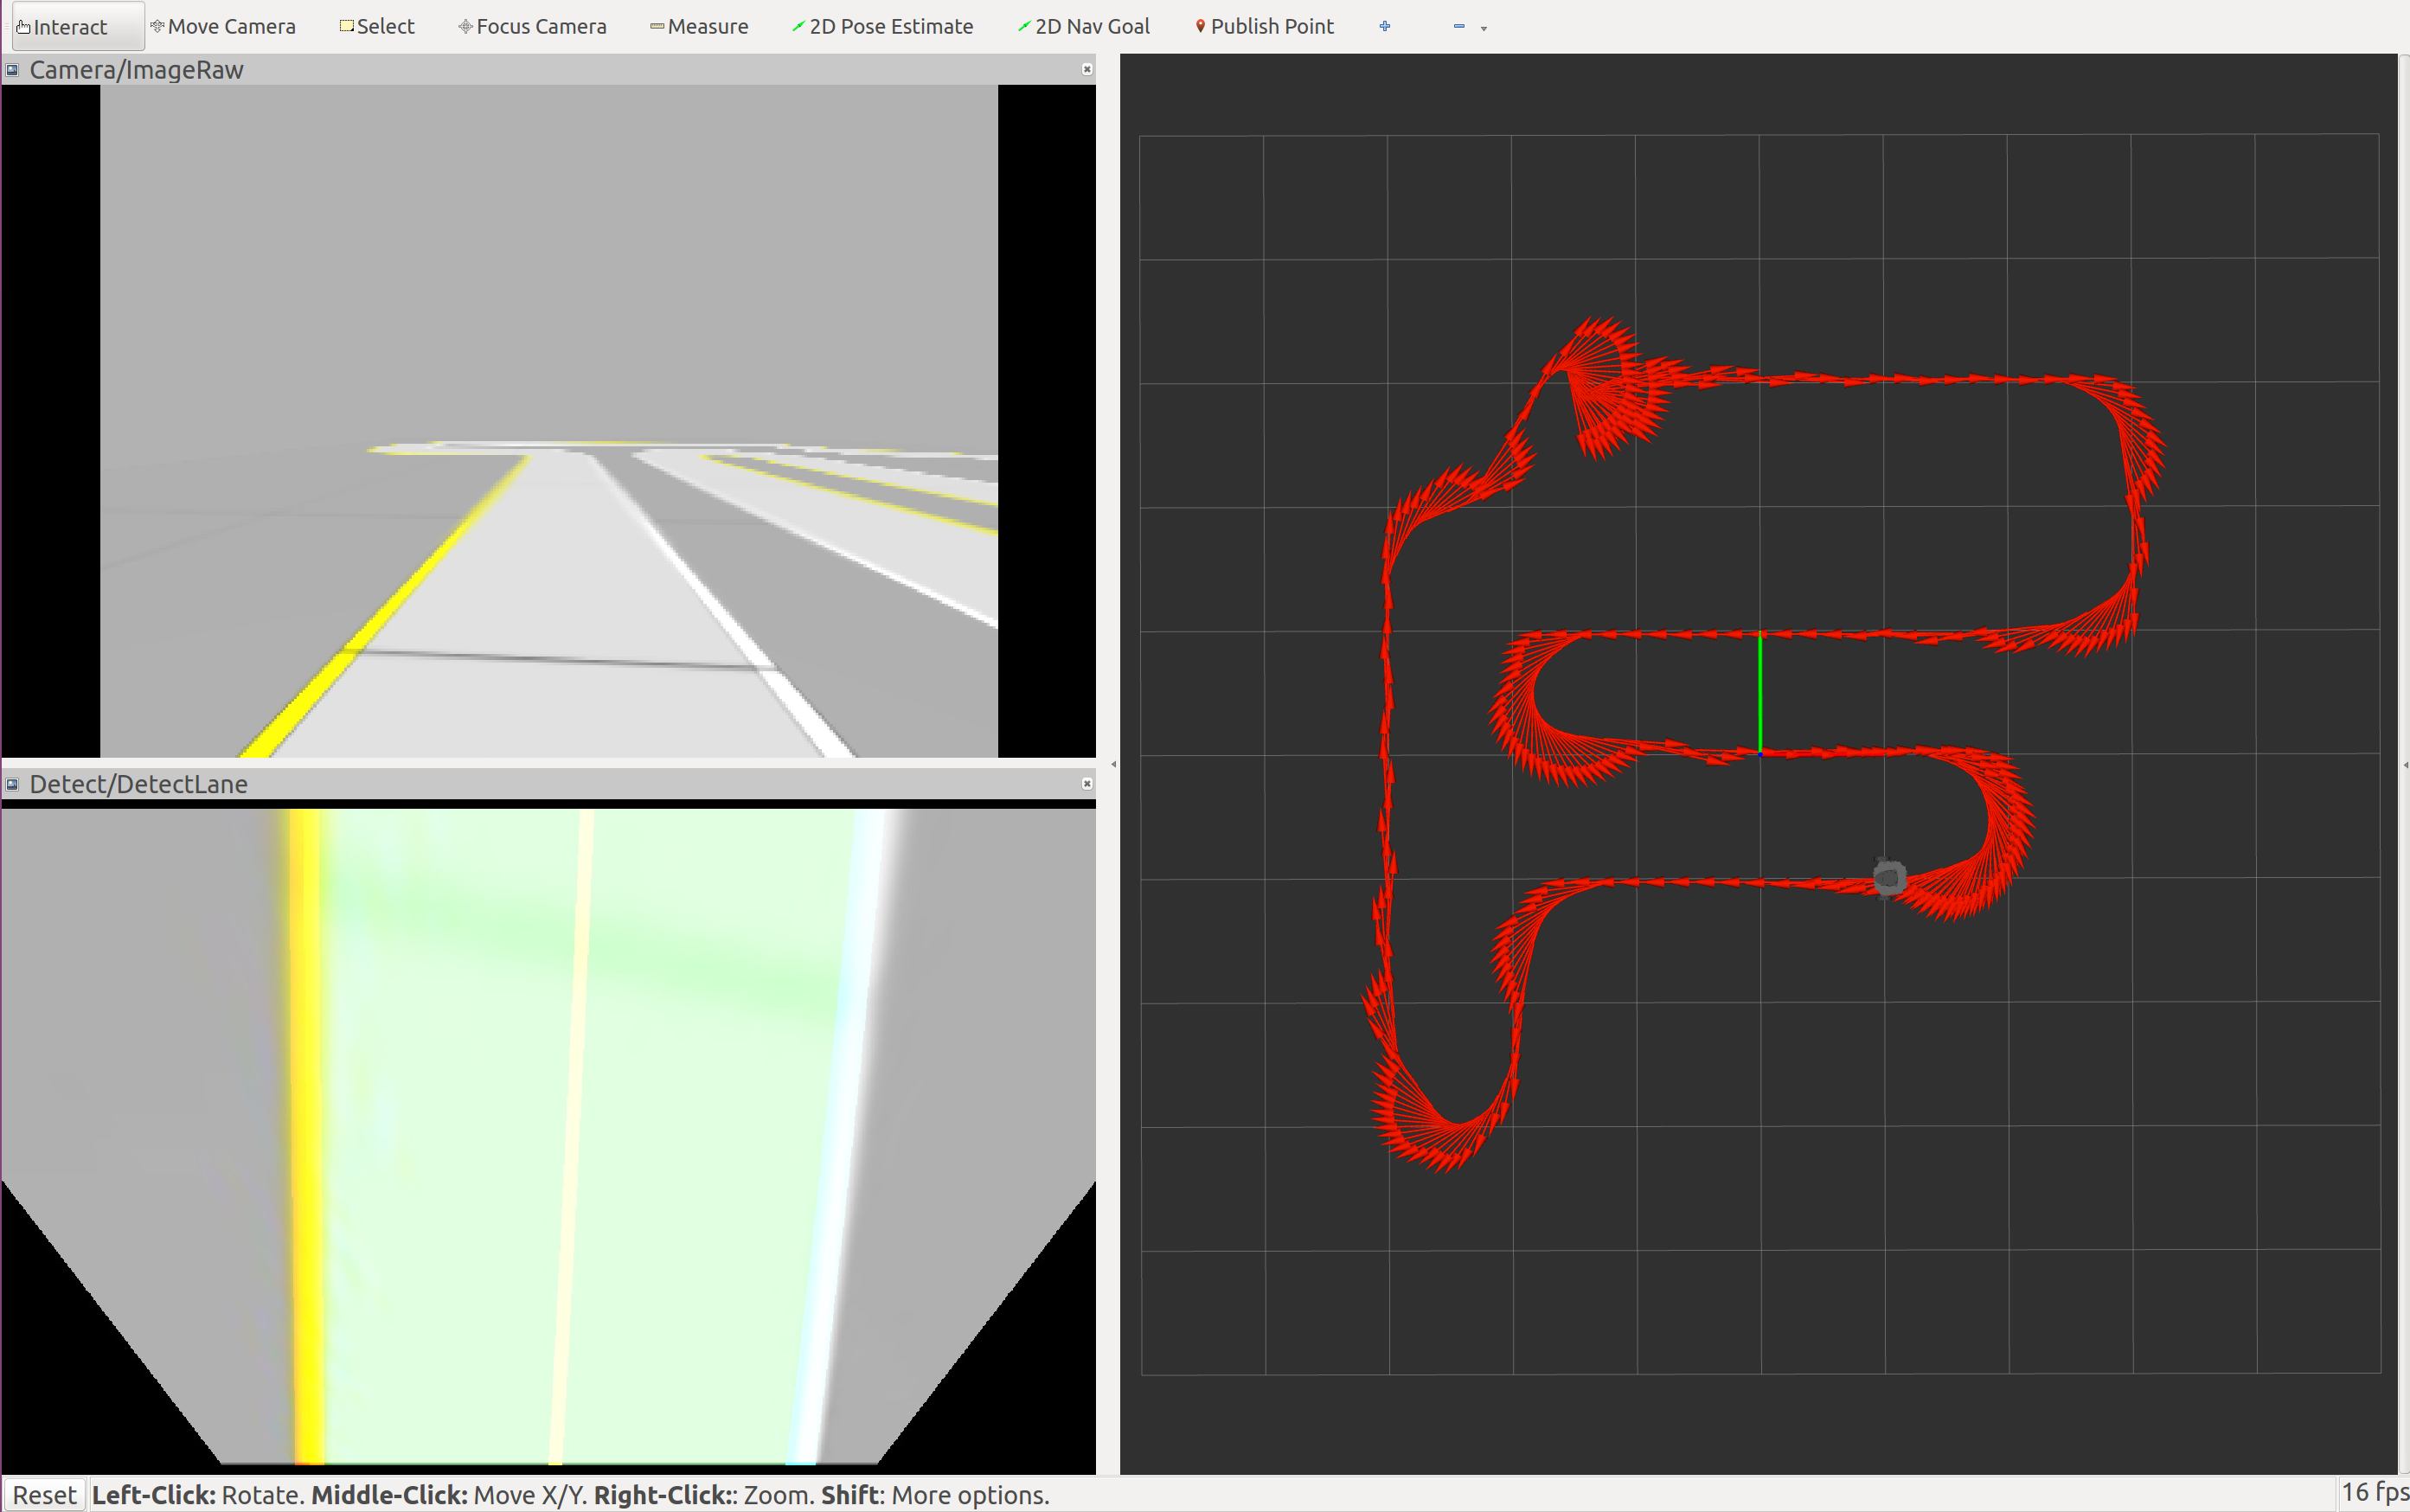
\includegraphics[width=0.65\textwidth]{figures/png/rviz}
\end{figure}

\end{frame}

	
\end{document}